%------------------------------------------------------------------------------------------------
\begin{minipage}{0.5\textwidth}
The figure to the right shows a crane whose cab \basis{A} supports a boom \basis{B} that swings
a wrecking ball $C_o$. This is the same setup from your homework.
\begin{enumerate}
\item Determine the angular velocity of \basis{B} in \basis{N}.
\\[2.0pc]
\item Determine the angular velocity of \basis{C} in \basis{N}.
\\[2.0pc]
\item Determine the angular velocity of \basis{C} in \basis{B}.
\\[4.0pc]
\end{enumerate}

\end{minipage}
\hfill
\begin{minipage}{0.48\textwidth}
\flushright
\vspace{-5.0pc}
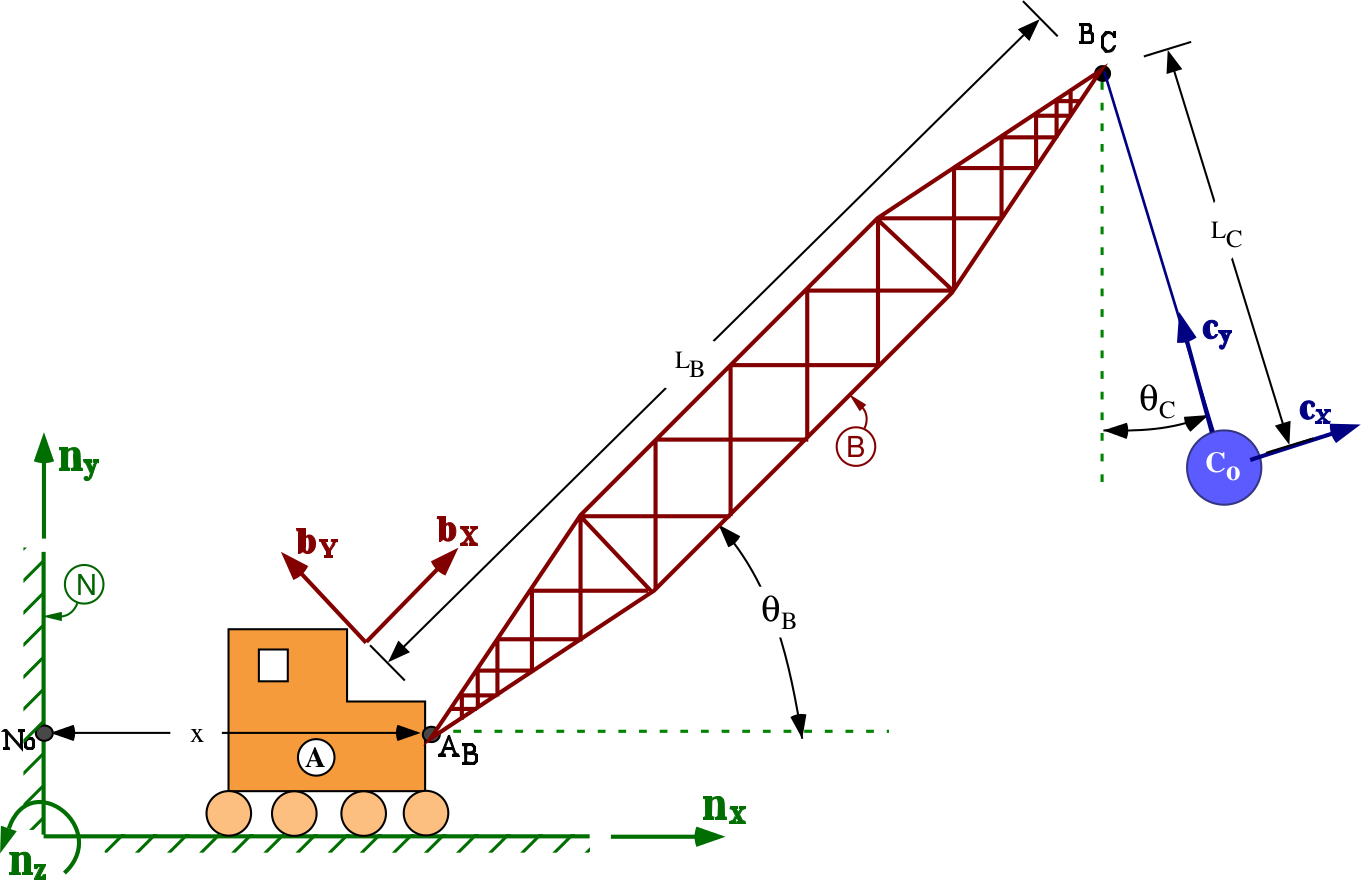
\includegraphics[width=\textwidth]{crane.png}
\end{minipage}